%%%%% SOME OPTIONS %%%%% 
\newcommand{\german}{false} % germanTrue or false --> Switch between german and english headers / titlepage
\newcommand{\coloredTitlePage}{true} % Switch between colored and BW titlepage
\newcommand{\company}{false}
\newcommand{\ECE}{true}
%%%%% Required Settings for the template %%%%%
%%%%% Configuration Package for the ThesisTemplate ECE / AEE %%%%%%
%
% Created by Mayer Florian October/2016
% v1.0

%======= DocumentClass ===========%
\documentclass[11pt, openright]{book} %Extarticle supports more FontSizes

%========= ADD Latex PACKAGES =========%
\usepackage{tabularx}         
\usepackage{parskip}%NEW
\newcolumntype{x}[1]{!{\centering\arraybackslash\vrule width #1}}
\usepackage{booktabs}
\usepackage[utf8]{inputenc} %to allow vowel mutations
\usepackage{tikz} % Schematic creator with TikZ in LaTex
\usepackage{geometry,titlesec,layout}
\usepackage{subfigure}
\usepackage{xcolor,colortbl}
%\usepackage{graphicx,rotating}
\usepackage{float}
\usepackage{epstopdf}
\usepackage[titles]{tocloft}
\usepackage{blindtext}
\usepackage{anyfontsize}
\usepackage{setspace,varwidth}
\usepackage{ifthen}
\usepackage{multicol,multirow}
\usepackage{makecell}
\usepackage[stable,bottom,hang,splitrule,multiple]{footmisc}% customize footnotes
\usepackage[final]{listings}% program code listings
\usepackage[%
headtopline,plainheadtopline,% activate all lines (header and footer)
headsepline,plainheadsepline,%
footsepline,plainfootsepline,%
footbotline,plainfootbotline,%
nouppercase% auto update \..mark
]{scrlayer-scrpage}% (KOMA)

\usepackage[%
breaklinks=true,% allow line break in links
colorlinks=true,% if false: framed link
linkcolor=black,anchorcolor=black,citecolor=black,filecolor=black,%
menucolor=black,urlcolor=black]{hyperref}% hyperlinks for references

\usepackage{amssymb}
\usepackage{emptypage}
\usepackage{glossaries}
\usepackage{appendix}
\usepackage{mdframed}
\usepackage{etoolbox}
\usepackage{chngcntr} 

\usepackage{textcomp}
\usepackage{lmodern}
\usepackage[european, straightvoltages, americaninductors, oldvoltagedirection]{circuitikz}

%========= ADD TikZ PACKAGES =========%
\usetikzlibrary{matrix,calc,positioning,arrows,shapes}
\usetikzlibrary{decorations.pathreplacing}

%======= END ADD PACKAGES =======%
\geometry{a4paper,twoside,%
	%textheight=205mm, %246mm,%
	textwidth=160mm,%
	top = 3cm,
	bottom = 4.5cm,
	heightrounded=false,% round textheight to multiple of lines (avoids overfull vboxes)
	ignoreall=true,% do not include header, footer, and margins in calculations
	marginparsep=5pt,% marginpar only used for signs (centered), thus only small sep. needed
	marginparwidth=10mm,% prevent margin notes to be out of page
	hmarginratio=1:2,
	voffset = 2.25mm,
	%headheight = 16mm,
	headsep = 9mm,
	footskip = 13mm
}
\linespread{1.4}
%======= DEFINE COLORS ===========%
\definecolor{DENcol}{RGB}{35,171,196} % Department Colour


%======= Re-Define Essential Commands and store old ones ======%
\newcommand{\ChapterFont}{qag}
\newcommand{\WorkingFont}{\rmdefault}
\renewcommand{\familydefault}{\WorkingFont}
\normalfont

%======= Set Depths of TOC / TOF / TOL =======%

\renewcommand{\cftchapfont}{\bf\large\fontfamily{\sfdefault}\selectfont}
\renewcommand{\cftpartfont}{\bf\large\fontfamily{\sfdefault}\selectfont}

\ifthenelse{\equal{\german}{true}}
{
\usepackage[ngerman]{babel}
\renewcommand{\lstlistingname}{Programmcode} 
}
%====== Usefull Additional Commands =======%

% Make clickable footnote
    \newcommand{\hyperfootnote}[1][]{\def\ArgI\hyperfootnoteRelay}
    % relay to new command to make extra optional command possible
    \newcommand\hyperfootnoteRelay[2][]{\href{#1#2}{\ArgI}\footnote{\href{#1#2}{#2}}}
    % the first optional argument is now in \ArgI, the second is in #1
    %http://www.brechtdeman.com/blog/latex-clickable-footnote.html
    % Simple (no arguments)
    %    \hyperfootnote{http://www.mywebsite.com}
    % Link text (1 argument)
    %   \hyperfootnote[My website]{http://www.mywebsite.com}
    % Link text and invisible prefix (2 arguments)
    %   \hyperfootnote[My website][http://]{www.mywebsite.com}

\newcommand{\ie}{i.\,e.}
\newcommand{\Ie}{I.\,e.}
\newcommand{\eg}{e.\,g.}
\newcommand{\Eg}{E.\,g.} 

%====== Heading Commands =======%

\pagestyle{scrheadings}%
% \setlength\parindent{0cm}% no indentation for first line of new paragraph
% \raggedbottom% do not try to fill pages

% header and footer size
\setheadwidth{text}% set header width to textwidth
\setfootwidth{text}% set footer width to textwidth
\setheadtopline[textwithmarginpar]{0.25pt}% set up separator lines (greater width than text)
\setheadsepline[textwithmarginpar]{0.25pt}
\setfootsepline[textwithmarginpar]{0.25pt}
\setfootbotline[textwithmarginpar]{0.25pt}

\renewcommand*\chaptermark[1]{\markleft{\thechapter~#1}}
\renewcommand*\sectionmark[1]{\markright{\thesection~#1}} 

\clearscrheadfoot % clear everything
\ihead[]{}%
\ohead[\ShortTitle]{\footnotesize\headmark}%
%\cfoot[\footnotesize\ConfidNote]{\footnotesize\ConfidNote}%

\ofoot[\ifthenelse{\equal{\thepage}{}}{\pagemark}{--~~\pagemark~~--}]{\ifthenelse{\equal{\thepage}{}}{\pagemark}{--~~\pagemark~~--}}%

%============== Chapter / Section / Subsection Style ==== %
\titleformat{\part}[display]
   {\fontfamily{\sfdefault}\bfseries\fontsize{26}{26}\selectfont\filcenter}
   {\fontfamily{\sfdefault}\bfseries\fontsize{30}{22}\selectfont\partname{} \thepart}
   {0.5em}
   {}

\titleformat{\chapter}[display]
{\fontfamily{\sfdefault}\bfseries\fontsize{22}{22}\selectfont}%\
{
\begin{tikzpicture}[overlay]
	\node (CoolTitle) at (12,1) [opacity=0.325]{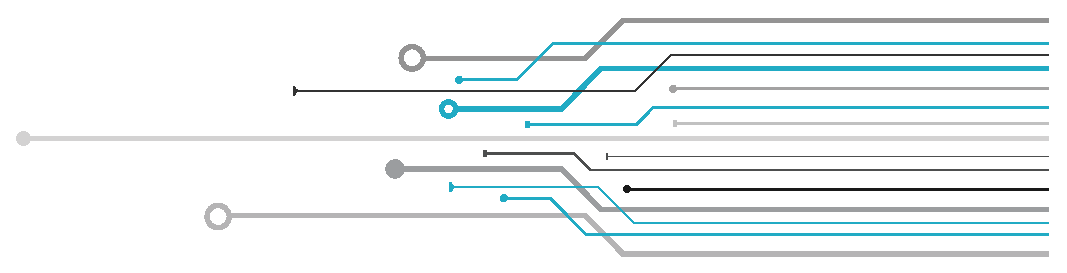
\includegraphics[scale=0.75]{temp_graphics/chapterBacking.eps}};
	\node (titleNumber) at ($(CoolTitle)+(3,0)$) {\textcolor{black!80}{\fontfamily{\ChapterFont}\bfseries\Large\fontsize{80}{80}\selectfont\thechapter}};
\end{tikzpicture}
}
{0.05em}%
{\vspace{0.25ex}\filleft}%

\titleformat{\section}{\Large \bfseries \sffamily}{\thesection}{1 em}{}
\titleformat{\subsection}{\large \bf \sffamily}{\thesubsection}{1 em}{}
\titleformat{\subsubsection}{\large \bf \sffamily}{\thesubsubsection}{1 em}{}

%%%% CLEAR DOUBLE-PAGE
% redefine cleardoublepage...
\makeatletter
\renewcommand{\cleardoublepage}{\clearpage\if@twoside\ifodd\c@page\else\thispagestyle{plain}\hbox{}\newpage\if@twocolumn\hbox{}\newpage\fi\fi\fi}
% ...and define empty double page (e.g., for title sheet)
\newcommand{\emptydoublepage}{\clearpage\if@twoside\ifodd\c@page\else\thispagestyle{empty}\hbox{}\newpage\if@twocolumn\hbox{}\newpage\fi\fi\fi}%
% ...and also an empty single page
\newcommand{\emptypage}{\clearpage\thispagestyle{empty}\hbox{}\newpage\if@twocolumn\hbox{}\newpage\fi}%
\makeatother

%%%%% Correct Even and Odd Pages %%%%%
\let\tmp\oddsidemargin
\let\oddsidemargin\evensidemargin
\let\evensidemargin\tmp
\reversemarginpar

% code listings
\lstloadlanguages{Bash,VHDL,Matlab,[ANSI]C,Java,[LaTeX]TeX}

\lstset{
	frame=top,frame=bottom,
	basicstyle=\fontsize{8}{8}\normalfont\sffamily,    % the size of the fonts that are used for the code
	stepnumber=1,                           % the step between two line-numbers. If it is 1 each line will be numbered
	numbersep=6pt,                         % how far the line-numbers are from the code
	tabsize=2,                              % tab size in blank spaces
	extendedchars=true,                     %
	breaklines=true,                        % sets automatic line breaking
	captionpos=t,                           % sets the caption-position to top
	mathescape=true,
	stringstyle=\color{black}\ttfamily, % Farbe der String
	showspaces=false,           % Leerzeichen anzeigen ?
	showtabs=false,             % Tabs anzeigen ?
	xleftmargin=15pt,
	framexleftmargin=14pt,
	framexrightmargin=9pt,
	framexbottommargin=5pt,
	framextopmargin=5pt,
	showstringspaces=false,      % Leerzeichen in Strings anzeigen ?
	numbers = left,
	linewidth = 150mm
}
%%%% MDBOX Setup
\mdfsetup{%
middlelinecolor=red,
middlelinewidth=2pt,
backgroundcolor=DENcol!10,
roundcorner=10pt,
topline = false,
bottomline = false,
rightline = false,
linecolor = DENcol,
linewidth = 10pt}

%%%% GET RID OF OVERFULL BOXING WARNINGS %%%%
%\overfullrule=5pt
\setlength{\headheight}{1.1\baselineskip}
\raggedbottom

%%%%%%%%%%%%%
\counterwithout{footnote}{chapter}


\usepackage{hyperref}

\makeglossaries

%\input{redCurrArrows.tex}

\makeatletter
\newcommand{\myscope}[2] % #1 = name , #2 = rotation angle
{\draw[thick,rotate=#2] (#1) circle (12pt)
 (#1) ++(-0.35,-0.1) -- ++(0.3,0.3) --++(0,-0.3)-- ++(0.3,0.3) --++(0,-0.3);
}
\newcommand{\costumPicWidth}[0]{
0.8\textwidth
}

\newcommand{\costumPlotWidth}[0]{
\textwidth
}

%\addto\extrasngerman{\def\figureautorefname{picture}}
%\addto\extrasngerman{\def\equationautorefname{equation}}
%\addto\extrasngerman{\def\tableautorefname{table}}

\newcommand{\V}[0]{\text{V}}
\newcommand{\mV}[0]{\text{mV}}
\newcommand{\uV}[0]{\mu\text{V}}

\newcommand{\A}[0]{\text{A}}
\newcommand{\mA}[0]{\text{mA}}
\newcommand{\uA}[0]{\mu\text{A}}

\newcommand{\s}[0]{\text{s}}
\newcommand{\ms}[0]{\text{ms}}
\newcommand{\us}[0]{\mu\text{s}}

\newcommand{\Ohms}[0]{\Omega}
\newcommand{\KOhms}[0]{\text{K}\Omega}
\newcommand{\MOhms}[0]{\text{M}\Omega}

\newcommand{\F}[0]{\text{F}}
\newcommand{\mF}[0]{\text{mF}}
\newcommand{\uF}[0]{\mu\text{F}}
\newcommand{\nF}[0]{\text{nF}}

\newcommand{\Hz}[0]{\text{Hz}}
\newcommand{\kHz}[0]{\text{kHz}}
\newcommand{\MHz}[0]{\text{MHz}}

\newcommand{\dB}[0]{\text{dB}}

\newcommand{\degree}[0]{^\circ}

\newcommand{\Mikro}[0]{\mu}
\newcommand{\Milli}[0]{\text{m}}
\newcommand{\Kilo}[0]{\text{k}}
\newcommand{\Mega}[0]{\text{M}}

\begin{document}
\lstset{language=Matlab,%
    %basicstyle=\color{red},
    breaklines=true,%
    morekeywords={matlab2tikz},
    keywordstyle=\color{blue},%
    morekeywords=[2]{1}, keywordstyle=[2]{\color{black}},
    identifierstyle=\color{black},%
    stringstyle=\color{mylilas},
    commentstyle=\color{mygreen},%
    showstringspaces=false,%without this there will be a symbol in the places where there is a space
    numbers=left,%
    numberstyle={\tiny \color{black}},% size of the numbers
    numbersep=9pt, % this defines how far the numbers are from the text
    emph=[1]{for,end,break},emphstyle=[1]\color{red}, %some words to emphasise
    %emph=[2]{word1,word2}, emphstyle=[2]{style},    
}

%%%%% ThesisTemplate ECE / AEE %%%%%%
%
% Created by Mayer Florian October/2016
% v1.0

%============== Glossary Command ==== %

\newglossaryentry{SCSS}{name=SCSS, description={Single Channel Source Separation}} 
\newglossaryentry{ITD}{name=ITD, description={Interaural Time Difference}}
\newglossaryentry{PASCSS}{name=PASCSS, description={Phase-Aware Single Channel Source Separation}}
\newglossaryentry{CASA}{name=CASA, description={Computational Auditory Scene Analysis}}
\newglossaryentry{NMF}{name=NMF, description={Non-Negative Matrix Factorization}}
\newglossaryentry{CMF}{name=CMF, description={Complex Matrix Factorization}}
\newglossaryentry{STFT}{name=STFT, description={Short-Time Fourier Transformation}}
\newglossaryentry{DTFT}{name=DTFT, description={Discrete-Time Fourier Transformation}}
\newglossaryentry{ISTFT}{name=ISTFT, description={Inverse Short-Time Fourier Transformation}}
\newglossaryentry{IBM}{name=IBM, description={Ideal Binary Mask}}
\newglossaryentry{IRM}{name=IRM, description={Ideal Ratio Mask}}
\newglossaryentry{SNR}{name=SNR, description={Signal-to-Noise Ratio}}
\newglossaryentry{DNN}{name=DNN, description={Deep neural network}}
\newglossaryentry{SVM}{name=SVM, description={Support vector machine}}
\newglossaryentry{KL-divergence}{name=KL-divergence, description={Kullback-Leibler divergence}}
\newglossaryentry{MPE}{name=MPE, description={Multipitch Estimator}} 
\newglossaryentry{PEFAC}{name=PEFAC, description={Pitch Estimation Filter with Amplitude Compression}}  
\newglossaryentry{GMM}{name=GMM, description={Gaussian mixture models}} 
\newglossaryentry{GLA}{name=GLA, description={Griffin and Lim Algorithm}}  
\newglossaryentry{MISI}{name=MISI, description={Multiple Input Spectrogram Inversion}}
\newglossaryentry{PPR}{name=PPR, description={Partial Phase Reconstruction}}
\newglossaryentry{ISSIR}{name=ISSIR, description={Partial Phase Reconstruction for Informed Source Separation}}
\newglossaryentry{FHMM}{name=FHMM, description={Factorial Hidden Markov Models}}
\newglossaryentry{HMM}{name=HMM, description={Hidden Markov Models}}
\newglossaryentry{SHR}{name=SHR, description={Subharmonic to harmonic ratio}}
\newglossaryentry{POC}{name=POC, description={Proof of Concept}}
\newglossaryentry{SSR}{name=SSR, description={Signal-to-Signal Ratio}}
\newglossaryentry{GPE}{name=GPE, description={Gross-Pitch Error}}
\newglossaryentry{MMSE}{name=MMSE, description={Minimum Mean Squared Error}}
\newglossaryentry{PESQ}{name=PESQ, description={Perceptual Evaluation of Speech Quality}}
\newglossaryentry{STOI}{name=STOI, description={Short-time objective intelligibility}}
\newglossaryentry{BSS-Eval}{name=BSS-Eval, description={Blind Source separation evaluation}}
\newglossaryentry{SDR}{name=SDR, description={Signal-to-Distortion Ratio}}
\newglossaryentry{SIR}{name=SIR, description={Signal-to-Interference Ratio}}
\newglossaryentry{SAR}{name=SAR, description={Signal-to-Artifact Ratio}}
\newglossaryentry{PE}{name=PE, description={Phase Estimation}}
\newglossaryentry{SSN}{name=SSN, description={Speech-Shaped Noise}}
%frontmatter inluding:
%titlepage, abstract, acknowledgments, declaration, toc, lof, lot
\frontmatter
\renewcommand{\thepage}{\Roman{page}}

% titlepage ----> changelog
%% Author: Mayer Florian (ECE)
%%
%% 10.10.16 ---------> Created TitlePage 

\renewcommand{\familydefault}{\sfdefault}
\normalfont 

%%%%% Now we add YOUR Personal DATA %%%%%
%%%%% What you enter here, will be written to the variables used within this document !! %%%%%%
\ifthenelse{\equal{\german}{true}}
{
	\newcommand{\ThesisTitle}{Analoge Signalverarbeitung}
	\newcommand{\ThesisSubtitle}{Laborprotokoll}
	\newcommand{\ShortTitle}{ASV Laborprotokoll} % needed for headers within your document 
	\newcommand{\ThesisAuthor}{Anderle Fabian, Grebien Alexander}
	\newcommand{\ThesisDate}{Graz, SS2020}
	\newcommand{\ThesisType}{} % Bachelor Thesis
	%\newcommand{\Organization}{am Bachelor Studiengang Elektronik und Computer Engineering \\ der FH JOANNEUM -- University of Applied Sciences, Austria}
	\newcommand{\Supervisor}{} % Supervisor 1 \\ Supervisor 2 \\ ...
	\newcommand{\CoSupervisor}{} % Supervisor 1 \\ Supervisor 2 \\ ...
	\newcommand{\Assessors}{}
	\newcommand{\SpecialNote}{}
	%%%%%%%%%%%%%%%%%%%%%%%%%%%%%%%%
}
{
	\newcommand{\ThesisTitle}{MBD Lab report}
	\newcommand{\ThesisSubtitle}{Solver development}
	\newcommand{\ShortTitle}{Model based design} % needed for headers within your document 
	\newcommand{\ThesisAuthor}{Grebien Alexander}
	\newcommand{\ThesisDate}{Graz, \today}
	\newcommand{\ThesisType}{} % Bachelor Thesis
	%\newcommand{\Organization}{am Bachelor Studiengang Elektronik und Computer Engineering \\ der FH JOANNEUM -- University of Applied Sciences, Austria}
	\newcommand{\Supervisor}{} % Supervisor 1 \\ Supervisor 2 \\ ...
	\newcommand{\CoSupervisor}{} % Supervisor 1 \\ Supervisor 2 \\ ...
	\newcommand{\Assessors}{}
	\newcommand{\SpecialNote}{}
}
%%%%%%%%%%%%%%%%%%%%%%%%%%%%%%%%

\ifthenelse{\equal{\coloredTitlePage}{true}}
{
\newcommand{\bcol}{DENcol}
\newcommand{\tcol}{white}
}{
\newcommand{\bcol}{white}
\newcommand{\tcol}{black}
}

\thispagestyle{empty}

%====== Create Sizes For Title what so ever ====== %
\newcommand{\MainTitlesize}{\bf\fontsize{24}{24}\selectfont}
\newcommand{\SubTitlesize}{\bf\fontsize{16}{16}\selectfont}
\newcommand{\Namesize}{\bf\fontsize{14}{14}\selectfont}

\ifthenelse{\equal{\german}{true}}
{
\begin{tikzpicture}[overlay]

\ifthenelse{\equal{\company}{true}}
{
	\ifthenelse{\equal{\ECE}{true}}
	{
		\node (Logo) at (9cm,-1) [anchor = east] {
\includegraphics[scale = 1]{temp_graphics/company_logo.eps}};
		\node (Logo2) at (17cm,-0.9) [anchor = east] {
\includegraphics[scale = 1.1]{temp_graphics/logo_FHJ_ECE_white.eps}};
	}
	{
		\node (Logo) at (9cm,-1) [anchor = east] {
\includegraphics[scale = 1]{temp_graphics/company_logo.eps}};
		\node (Logo2) at (17cm,-0.9) [anchor = east] {
\includegraphics[scale = 1.1]{temp_graphics/ecm_logo_eps.eps}};
	}
}
{
	\ifthenelse{\equal{\ECE}{true}}
	{
		\node (Logo) at (17cm,-0.9) [anchor = east] {
\includegraphics[scale = 1.1]{temp_graphics/logo_FHJ_ECE_white.eps}};
	}
	{
		\node (Logo) at (16cm,-0.9) [anchor = east] {
\includegraphics[scale = 0.9]{temp_graphics/ecm_logo_eps.eps}};
	}
}

%% ===== CREATE background ===== %%
% Background Box
\node (boxOne)  at (7cm,-12) [minimum width=1.1\paperwidth,fill = \bcol, minimum height=18cm, inner sep=0pt] {};

\node (ThesisTitle) [color = \tcol, font = \MainTitlesize, align = flush right, anchor = north east] at (16,-4){\ThesisTitle};

\node (ThesisSubtitle) [color = \tcol, font = \SubTitlesize, align = flush right, anchor = north east] at ($(ThesisTitle.south east) + (0,-0.25em)$){\ThesisSubtitle};

\node (ThesisType) [color = \tcol, font = \SubTitlesize, align = flush right, anchor = north east] at ($(ThesisSubtitle.south east) + (0,-3em)$){\ThesisType};

\node (AuthName) [color = \tcol, font = \large, align = flush right, anchor = north east] at ($(ThesisType.south east) + (0,-2em)$){\bf{angefertigt von:} \\ \ThesisAuthor};



\ifthenelse{\equal{\ECE}{true}}
{
	\node (Organization) [color = \tcol, font = \large, align = flush right, anchor = north east] at ($(AuthName.south east) + (0,-3em)$){am Bachelor-Studiengang Elektronik und Computer Engineering \\ der FH JOANNEUM -- University of Applied Sciences, Austria};
}
{
	\node (Organization) [color = \tcol, font = \large, align = flush right, anchor = north east] at ($(AuthName.south east) + (0,-3em)$){am Master-Studiengang Electronics and Computer Engineering \\ der FH JOANNEUM -- University of Applied Sciences, Austria};
}

\node (Supervisor) [color = \tcol, font = \large, align = flush right, anchor = north east] at ($(Organization.south east) + (0,-3em)$){\bf{ } \\ \Supervisor};

\ifthenelse{\equal{\company}{true}}
{
	\node (COSupervisor) [color = \tcol, font = \large, align = flush right, anchor = north east] at ($(Supervisor.south east) + (0,-3em)$){\bf{extern Betreut von:} \\ \CoSupervisor};
	
	\node (ThesisDate) [color = \tcol, font = \large, align = flush right, anchor = north east] at ($(COSupervisor.south east) + (0,-3em)$){\bf\ThesisDate};
}
{

\node (ThesisDate) [color = \tcol, font = \large, align = flush right, anchor = north east] at ($(Supervisor.south east) + (0,-3em)$){\bf\ThesisDate};

}

\node (SpecialNote) [color = \tcol, font = \large, align = center, anchor = north east] at ($(ThesisDate.south east) + (0,-3em)$){\begin{varwidth}{14cm} \SpecialNote \end{varwidth}};

\end{tikzpicture}	
}
{
\begin{tikzpicture}[overlay]

\ifthenelse{\equal{\company}{true}}
{
	\ifthenelse{\equal{\ECE}{true}}
	{
		\node (Logo) at (9cm,-1) [anchor = east] {
\includegraphics[scale = 1]{temp_graphics/company_logo.eps}};
		\node (Logo2) at (17cm,-0.9) [anchor = east] {
\includegraphics[scale = 1.1]{temp_graphics/logo_FHJ_ECE_white.eps}};
	}
	{
		\node (Logo) at (9cm,-1) [anchor = east] {
\includegraphics[scale = 1]{temp_graphics/company_logo.eps}};
		\node (Logo2) at (17cm,-0.9) [anchor = east] {
\includegraphics[scale = 1.1]{temp_graphics/ecm_logo_eps.eps}};
	}
}
{
	\ifthenelse{\equal{\ECE}{true}}
	{
		\node (Logo) at (17cm,-0.9) [anchor = east] {
\includegraphics[scale = 1.1]{temp_graphics/logo_FHJ_ECE_white.eps}};
	}
	{
		\node (Logo) at (16cm,-0.9) [anchor = east] {
\includegraphics[scale = 0.9]{temp_graphics/ecm_logo_eps.eps}};
	}
}

%% ===== CREATE background ===== %%
% Background Box
\node (boxOne)  at (7cm,-12) [minimum width=1.1\paperwidth,fill = \bcol, minimum height=18cm, inner sep=0pt] {};

\node (ThesisTitle) [color = \tcol, font = \MainTitlesize, align = flush right, anchor = north east] at (16,-4){\ThesisTitle};

\node (ThesisSubtitle) [color = \tcol, font = \SubTitlesize, align = flush right, anchor = north east] at ($(ThesisTitle.south east) + (0,-0.25em)$){\ThesisSubtitle};

\node (ThesisType) [color = \tcol, font = \SubTitlesize, align = flush right, anchor = north east] at ($(ThesisSubtitle.south east) + (0,-3em)$){\ThesisType};

\node (AuthName) [color = \tcol, font = \large, align = flush right, anchor = north east] at ($(ThesisType.south east) + (0,-2em)$){\bf{created by:} \\ \ThesisAuthor};

\ifthenelse{\equal{\ECE}{true}}
{
	\node (Organization) [color = \tcol, font = \large, align = flush right, anchor = north east] at ($(AuthName.south east) + (0,-3em)$){at the bachelor degree programme Elektronik und Computer Engineering \\ of FH JOANNEUM -- University of Applied Sciences, Austria};
}
{
	\node (Organization) [color = \tcol, font = \large, align = flush right, anchor = north east] at ($(AuthName.south east) + (0,-3em)$){at the masters degree programme Elektronics and Computer Engineering \\ of FH JOANNEUM -- University of Applied Sciences, Austria};	
}

\node (Supervisor) [color = \tcol, font = \large, align = flush right, anchor = north east] at ($(Organization.south east) + (0,-3em)$){\bf{supervised by:} \\ \Supervisor};

\ifthenelse{\equal{\company}{true}}
{
	\node (COSupervisor) [color = \tcol, font = \large, align = flush right, anchor = north east] at ($(Supervisor.south east) + (0,-3em)$){\bf{external supervisor:} \\ \CoSupervisor};
	
	\node (ThesisDate) [color = \tcol, font = \large, align = flush right, anchor = north east] at ($(COSupervisor.south east) + (0,-3em)$){\bf\ThesisDate};
}
{
	\node (ThesisDate) [color = \tcol, font = \large, align = flush right, anchor = north east] at ($(Supervisor.south east) + (0,-3em)$){\bf\ThesisDate};
}

%\node (Assessor) [color = \tcol, font = \large, align = flush right, anchor = north east] at ($(Supervisor.south east) + (0,-3em)$){\bf{Prüfer:} \\ \Assessors};

\node (SpecialNote) [color = \tcol, font = \large, align = center, anchor = north east] at ($(ThesisDate.south east) + (0,-3em)$){\begin{varwidth}{14cm} \SpecialNote \end{varwidth}};

\end{tikzpicture}	
}
\renewcommand{\familydefault}{\WorkingFont}
\normalfont


\tableofcontents
\printglossary
%mainmatter inluding: Parts, chapters, sections, appendicies
\mainmatter
%Hier die verschiedenn tex_Dokumente der Labore einfügen
\chapter{Program architecture}
\section{Solver}

\section{Equations}

\chapter{Results}


\newpage
\chapter{Signaturen}
    Fertig gestellt am \today \\
    \begin{figure}[H]
        \centering
        
\includegraphics{pics/signature_grebien.png}
    	\caption{Signatur: Grebien Alexander}
    	\label{pic:signatur_grebien}
    \end{figure}
        
\listoffigures
\listoftables
\bibliographystyle{ieeetr}
\bibliography{meine_Zitatsbibliothek.bib}
\end{document}